\documentclass[8pt,a4paper,compress]{beamer}

\usepackage{/home/siyer/lib/slides}

\title{Compilation}
\date{}

\begin{document}
\begin{frame}
\vfill
\titlepage
\end{frame}

\begin{frame}
\frametitle{Outline}
\tableofcontents
\end{frame}

\section{Compilers}
\begin{frame}[fragile]
\pause

A compiler is a program that translates a source program written in a high-level programming language such as Java, C\lstinline{#} or C, into a target program in a lower level language such as machine code

\begin{center}
\visible<2->{
\includegraphics[scale=0.6]{{figures/figure01.01}.jpg}}
\end{center}

\pause
\bigskip

A programming language is an artificial language in which a programmer writes a program to control the behavior of a computer

\pause
\bigskip

Like a natural language, in a programming language, one describes
\begin{itemize}
\item The tokens (aka lexemes)

\item The syntax of programs and language constructs such as classes, methods, statements and expressions

\item The meaning (aka semantics) of the various constructs
\end{itemize}
\end{frame}

\begin{frame}[fragile]
\pause

A computer's machine language (ie, its instruction set) is designed so as to be easily interpreted by the computer itself

\pause
\bigskip

A machine's instruction set and its behavior is often referred to as its architecture

\pause
\bigskip

Examples of architectures
\begin{itemize}
\item Intel i386, a complex instruction set computer (CISC) with powerful and complex instructions

\item MIPS, as a reduced instruction set computer (RISC) with relatively simple instructions

\item Java Virtual Machine (JVM), a virtual machine not necessarily implemented in hardware
\end{itemize}

\pause
\bigskip

Traditionally, a compiler analyzes the input program to produce (or synthesize) the output program
\begin{itemize}
\item mapping names to memory addresses, stack frame offsets, and registers,

\item generating a linear sequence of machine code instructions, and

\item detecting any errors in the program that can be detected in compilation
\end{itemize}
\end{frame}

\begin{frame}[fragile]
\pause

An interpreter executes a high-level language program directly, ie, the high-level program is first loaded into the interpreter, and then executed

\begin{center}
\visible<2->{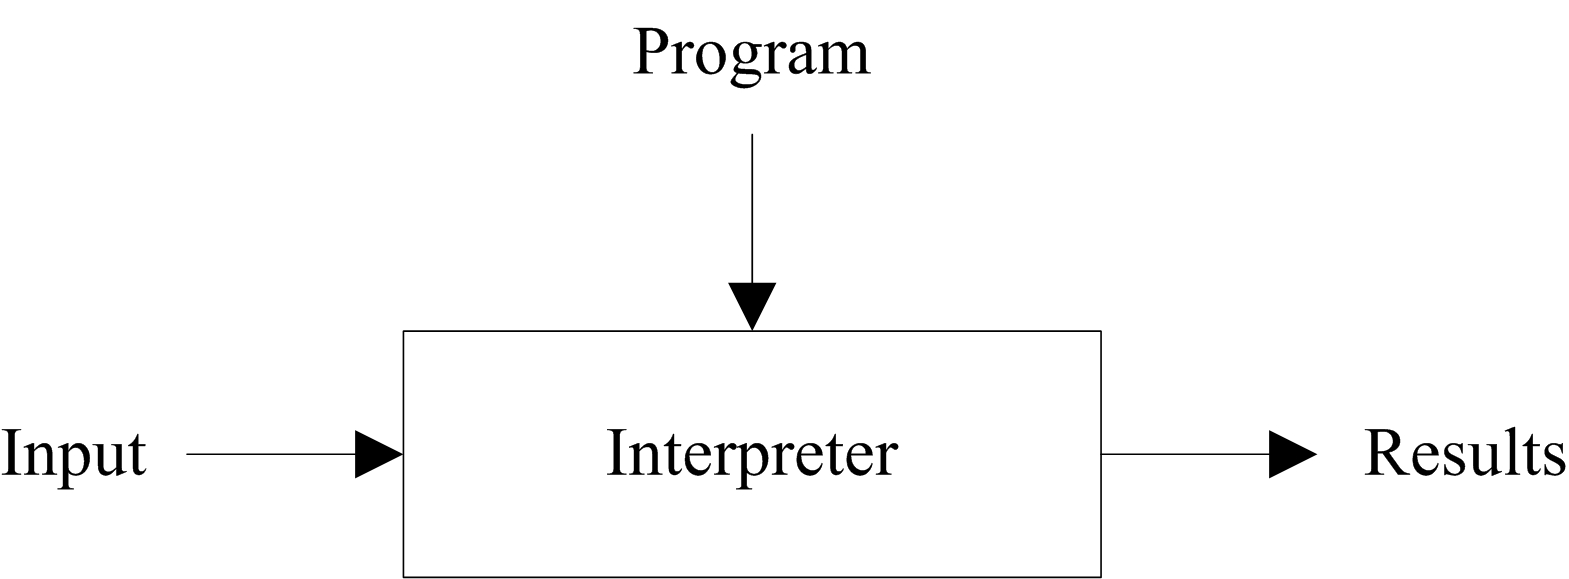
\includegraphics[scale=0.6]{{figures/figure01.02}.jpg}}
\end{center}

\pause
\bigskip

Examples of programming languages whose programs may be interpreted directly are the UNIX shell languages, such as bash and csh, Python, and many versions of LISP
\end{frame}

\section{Why Study Compilers?}
\begin{frame}[fragile]
\pause

Reasons for studying compilers
\begin{itemize}
\item Compilers are larger programs than the ones you have written in your programming courses

\item Compilers make use of all those things you have learned about earlier: arrays, lists, queues, stacks, trees, graphs, maps, regular expressions and finite state automata, context-free grammars and parsers, recursion and patterns

\item You learn a lot about the language you are compiling (in our case, Java)

\item You learn a lot about the target machine (in our case, both the Java Virtual Machine and the MIPS computer)

\item Compilers are still being written for new languages and targeted to new computer architectures

\item There is a good mix of theory and practice, and each is relevant to the other

\item The organization of a compiler is such that it can be written in stages, and each stage makes use of earlier stages; compiler writing is a case study in software engineering

\item Compilers are programs and writing programs is fun
\end{itemize}
\end{frame}

\section{The Phases of Compilation}
\begin{frame}[fragile]
\pause

At the very least, a compiler can be broken into a front end and a back end

\begin{center}
\visible<2->{
\includegraphics[scale=0.6]{{figures/figure01.03}.jpg}}
\end{center}

\pause
\bigskip

The front end takes as input, a high-level language program, and produces as output an intermediate representation (IR) of that program

\pause
\bigskip

The back end then takes the IR of the program as input, and produces the target machine language program
\end{frame}

\begin{frame}[fragile]
\pause

A compiler's front end analyzes the input program to determine its meaning, and so is source language dependent and target language independent

\pause
\bigskip

The front end can be further decomposed into a sequence of analysis phases

\begin{center}
\visible<2->{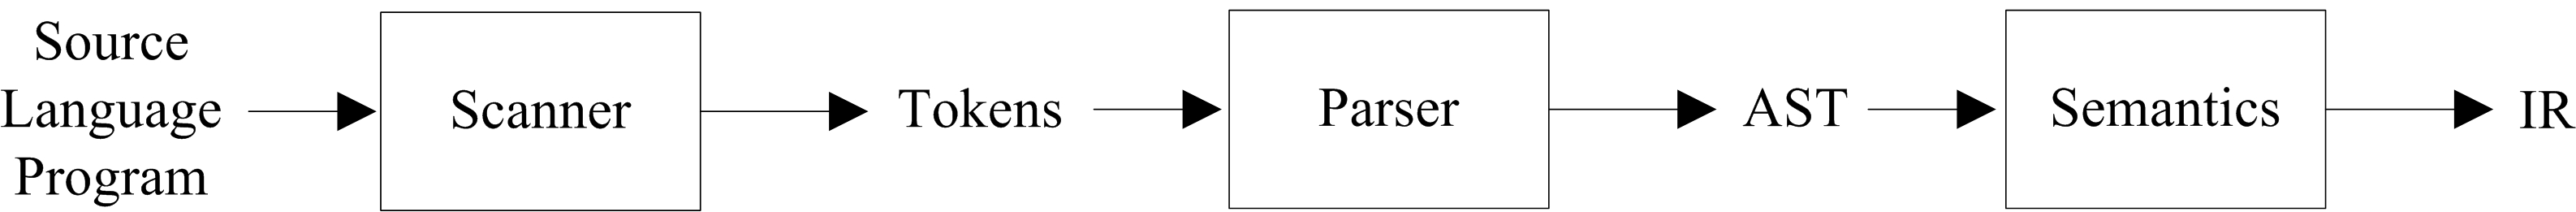
\includegraphics[scale=0.6]{{figures/figure01.04}.jpg}}
\end{center}

\pause
\bigskip

The scanner breaks the input stream of characters to a stream of tokens: identifiers, literals, reserved words, (one-, two-, three-, and four-character) operators
and separators

\pause
\bigskip

The parser takes a sequence of tokens and parses it against a grammar to produce an abstract syntax tree (AST), which makes the syntax that is implicit in the source program, explicit

\pause
\bigskip

The semantics phase does semantic analysis: declares names in a symbol table, looks up names as they are referenced to determine their types, assigns types to expressions, and checks the validity of types; sometimes, a certain amount of storage analysis (such as assigning addresses or offsets to variables) is also done
\end{frame}

\begin{frame}[fragile]
\pause

A compiler's back end takes the IR and produces (synthesizes) a target machine program having the same meaning, and so is target language dependent and source language independent

\pause
\bigskip

The back end can be further decomposed into a sequence of synthesis phases

\begin{center}
\visible<2->{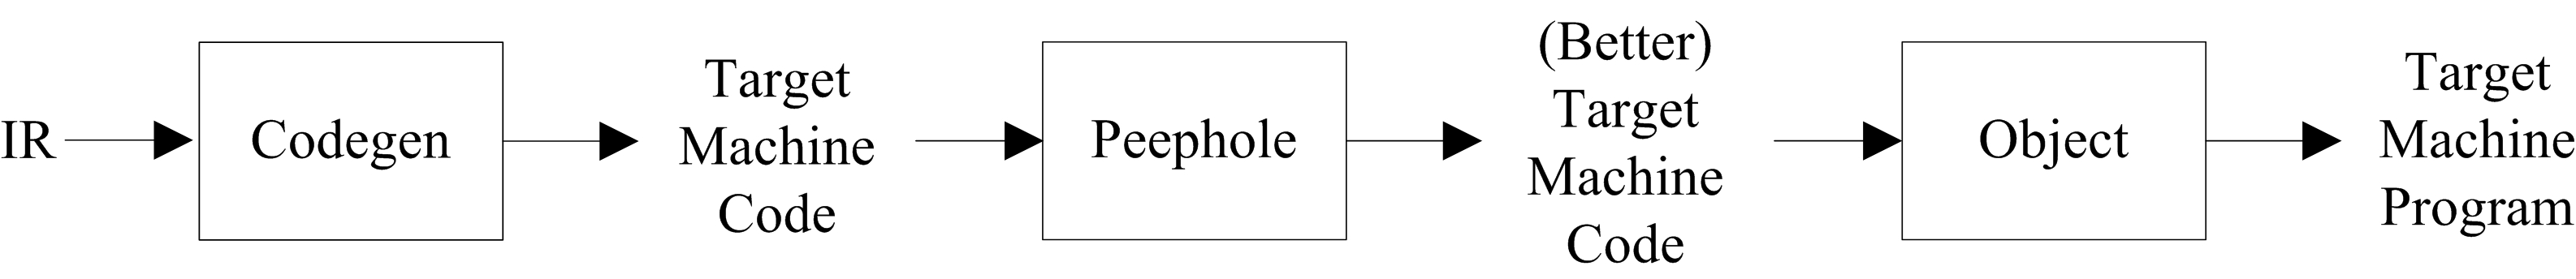
\includegraphics[scale=0.6]{{figures/figure01.05}.jpg}}
\end{center}

\pause
\bigskip

The code generation phase chooses what target machine instructions to generate, making use of information collected in earlier phases

\pause
\bigskip

The peephole phase scans through the generated instructions looking locally for wasteful instruction sequences such as branches to branches and unnecessary load/store pairs

\pause
\bigskip

The object phase links together any modules produced in code generation and it constructs a single machine code executable program
\end{frame}

\begin{frame}[fragile]
\pause

Sometimes, a compiler will have an optimizer (``middle end''), which sits between the front end and the back end

\begin{center}
\visible<2->{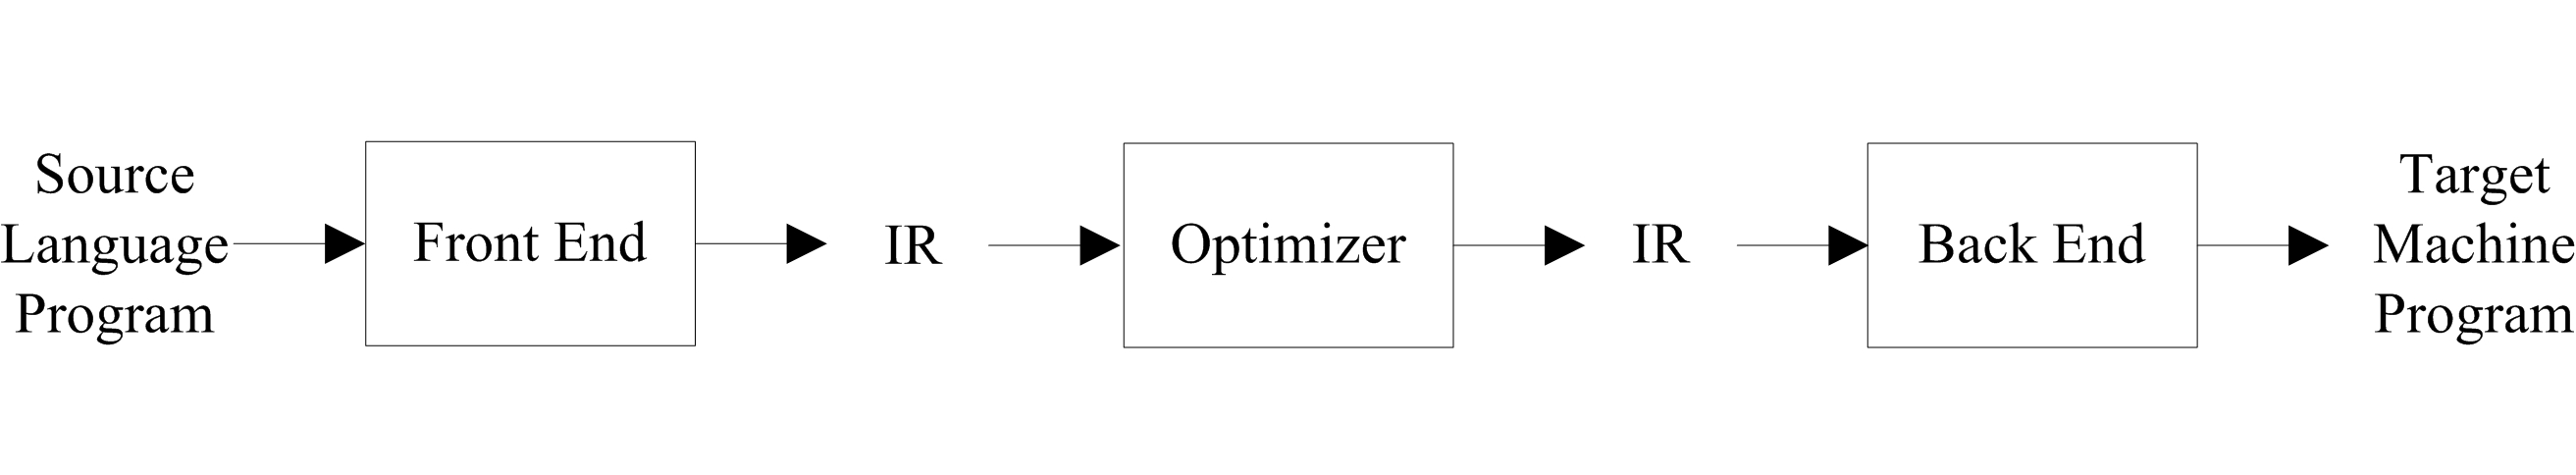
\includegraphics[scale=0.6]{{figures/figure01.06}.jpg}}
\end{center}

\pause
\bigskip

The purpose of the optimizer is both to improve the IR program and to collect information
that the back end may use for producing better code

\pause
\bigskip

The optimizer might do any number of the following
\begin{itemize}
\item Organize the program into what are called basic blocks: blocks of code from
which there are no branches out and into which there are no branches

\item From the basic block structure, one may then compute next-use information for determining the lifetimes of variables, and gather loop information

\item Next-use information is useful for eliminating common sub-expressions and constant folding (for example, replacing \lstinline{x + 5} by \lstinline{9} if we know \lstinline{x} has the value \lstinline{4})

\item Loop information is useful for pulling loop invariants out of loops and for strength reduction (for example, replacing multiplication operations by addition operations)
\end{itemize}
\end{frame}

\begin{frame}[fragile]
\pause

There are several advantages to separating the front end from the back end:
\begin{enumerate}
\item Decomposition reduces complexity; it's easier to understand (and implement) the smaller programs

\item Decomposition makes it possible for several individuals or teams to work concurrently on separate parts, reducing the overall implementation time

\item Decomposition permits a certain amount of code re-use; for example, once one has written
a front end for Java and a back end for the Intel Core Duo, one need only write a new C front end to get a C compiler, and one need only write a single SPARC back end to re-target both compilers to the Oracle SPARC architecture

\begin{center}
\visible<2->{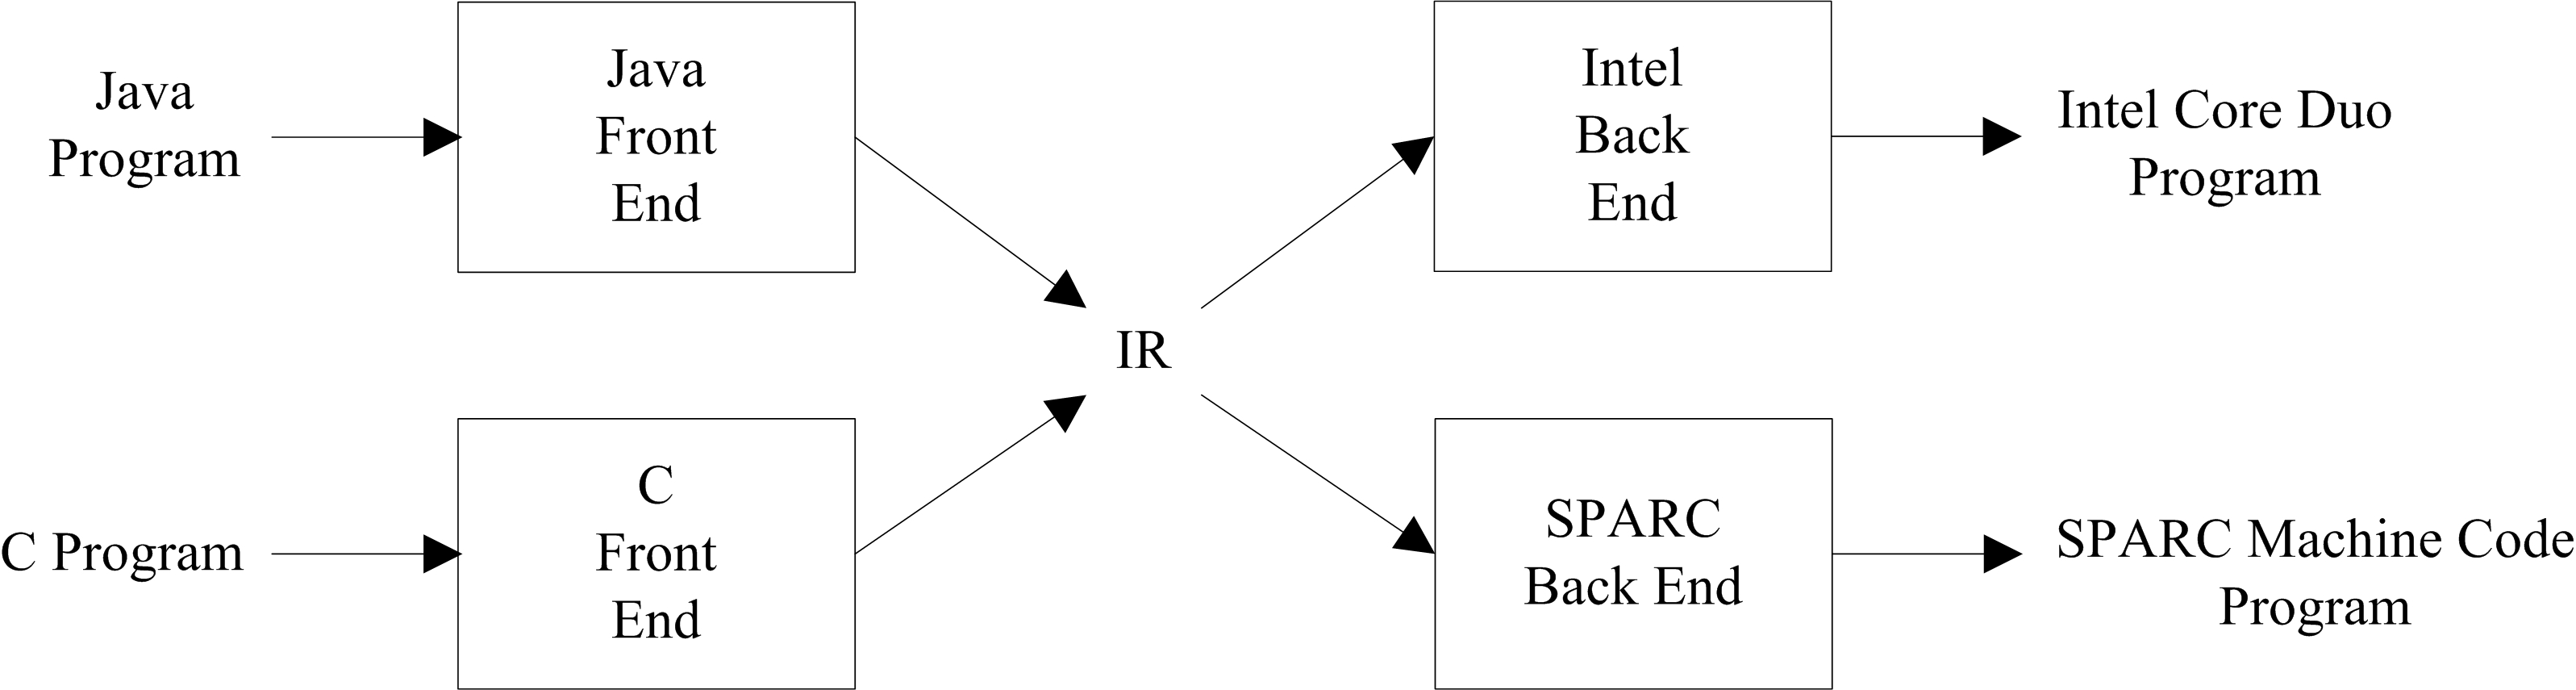
\includegraphics[scale=0.6]{{figures/figure01.07}.jpg}}
\end{center}
\end{enumerate}
\end{frame}

\begin{frame}[fragile]
\pause

The Java compiler, the program invoked when one types, for example
\begin{lstlisting}[language={}]
$ javac MyProgram.java
\end{lstlisting}
produces a \lstinline{MyProgram.class} file, a byte code program suitable for execution on the JVM

\pause
\bigskip

To execute the \lstinline{MyProgram.class} file, one types
\begin{lstlisting}[language={}]
$ java MyProgram
\end{lstlisting}
which effectively interprets the JVM program

\pause
\bigskip

In this course, we'll study the implementation of a compiler called \jmm to compile a (non-trivial) subset of Java, which we also call \jmm

\pause
\bigskip

In the first instance, we'll target the JVM

\pause
\bigskip

Targeting the JVM is deficient in one respect: one does not learn about register allocation because the JVM is a stack-based architecture and has no registers

\pause
\bigskip

To remedy this deficiency, we'll also study the compilation of JVM code to code for the MIPS machine, which is a register-based architecture; in doing this, we face the challenge of mapping possibly many variables to a limited number of fast registers
\end{frame}

\section{Overview of the \protect \jmm to JVM Compiler}
\begin{frame}[fragile]
\pause


\end{frame}

\section{The \protect \jmm Compiler Source Tree}
\begin{frame}[fragile]
\pause


\end{frame}
\end{document}
